\section{Results}
The parameters used in the simulation of a spiral galaxy are shown in \autoref{tab:galaxy-parameters}.
\begin{table}[htp]
    \centering
    \begin{tabular}{|l|c|}
        \hline
        \textbf{Parameter}      & \textbf{Value}           \\
        \hline
        Halo radius             & 3 kpc                    \\
        Halo mass               & $60 \times 10^9 M_\odot$ \\
        Disk radius             & 15 kpc                   \\
        Disk mass               & $15 \times 10^9 M_\odot$ \\
        Disk thickness          & 0.3 kpc                  \\
        Disk density profile    & Uniformly decreasing     \\
        Mass assignment scheme  & TSC                      \\
        Finite difference       & Two-point                \\
        Time integration method & Leapfrog                 \\
        \hline
    \end{tabular}
    \caption{Galaxy model parameters used in the simulation.}
    \label{tab:galaxy-parameters}
\end{table}
The galaxy is simulated as an isolated system, however, in deriving \autoref{eq:poisson-fourier-product}, periodic boundary conditions were assumed.
The simplest way (and the one used) to obtain a free-space solution from the PM method is to extend the computational domain twice in every dimension and fill the space unused in mass distribution with zeros.
The total size of the potential mesh used was $128 \times 128 \times 64$ with the region of interest occupying a box of size $60\, \text{kpc}\times 60\, \text{kpc}\times 30\, \text{kpc}$ located in a $64 \times 64 \times 32$ octant of the mesh.

\subsection{Particle-mesh method}
In the PM method, $N=50,000$ particles were used.
Cell size $H$ and time-step length were set to $60/64=0.9375$ kpc, and 1 Myr respectively.
The system's evolution over 200 Myr is shown in \autoref{fig:spiral-galaxy-evolution-pm}.

\begin{figure}[htp]
    \centering
    \begin{subfigure}[b]{0.45\textwidth}
        \centering
        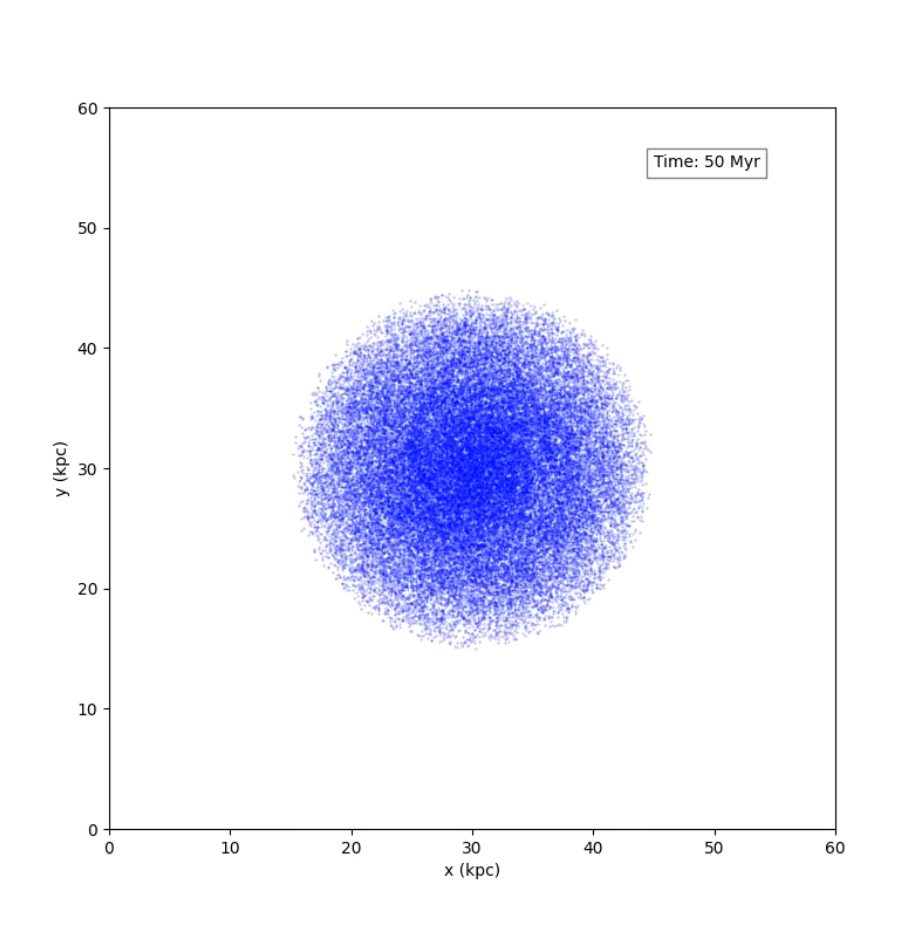
\includegraphics[width=\textwidth]{img/pm/50myr.png}
        \caption{$t=50\,\text{Myr}$}
        \label{fig:spiral-galaxy-evolution-pm-sub1}
    \end{subfigure}
    \hfill
    \begin{subfigure}[b]{0.45\textwidth}
        \centering
        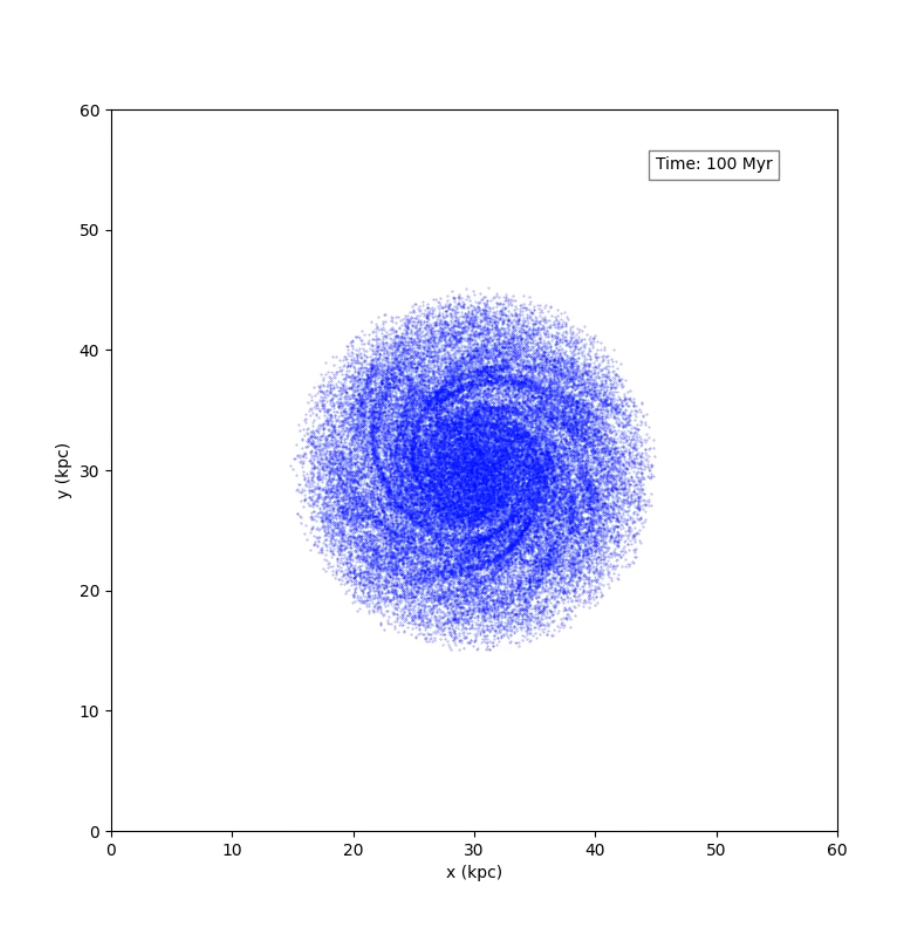
\includegraphics[width=\textwidth]{img/pm/100myr.png}
        \caption{$t=100\,\text{Myr}$}
        \label{fig:spiral-galaxy-evolution-pm-sub2}
    \end{subfigure}

    \vspace{0.5cm}

    \begin{subfigure}[b]{0.45\textwidth}
        \centering
        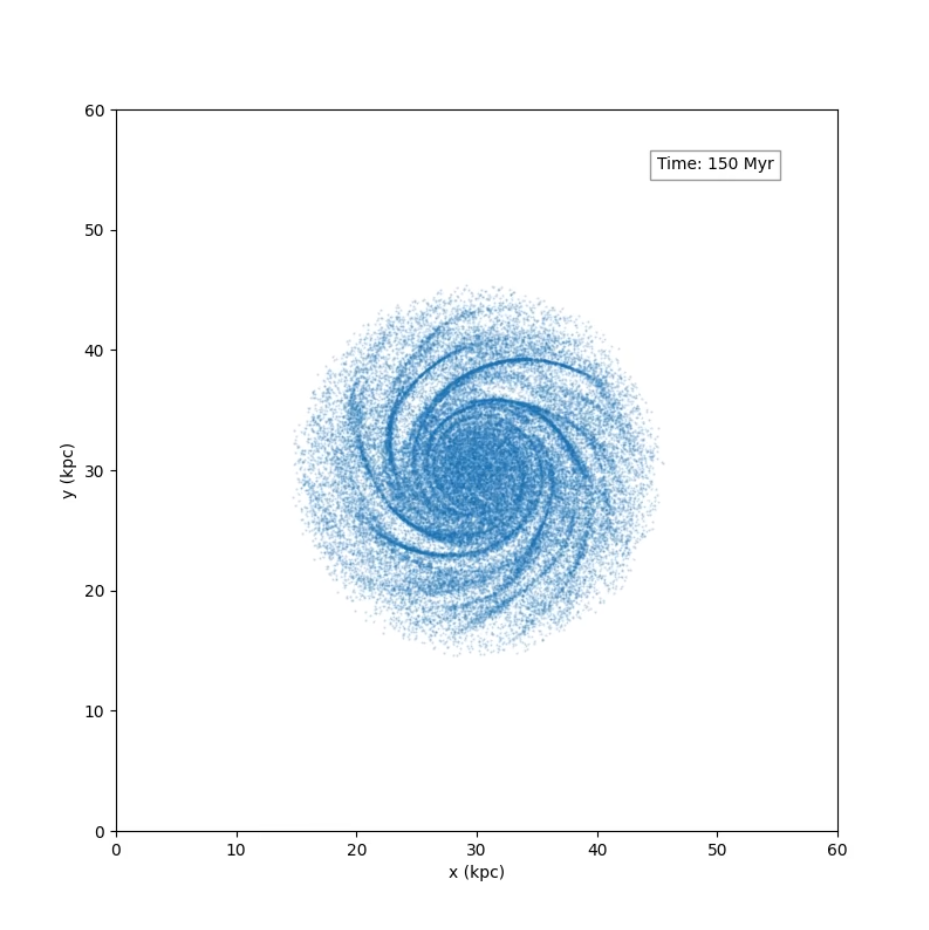
\includegraphics[width=\textwidth]{img/pm/150myr.png}
        \caption{$t=150\,\text{Myr}$}
        \label{fig:spiral-galaxy-evolution-pm-sub3}
    \end{subfigure}
    \hfill
    \begin{subfigure}[b]{0.45\textwidth}
        \centering
        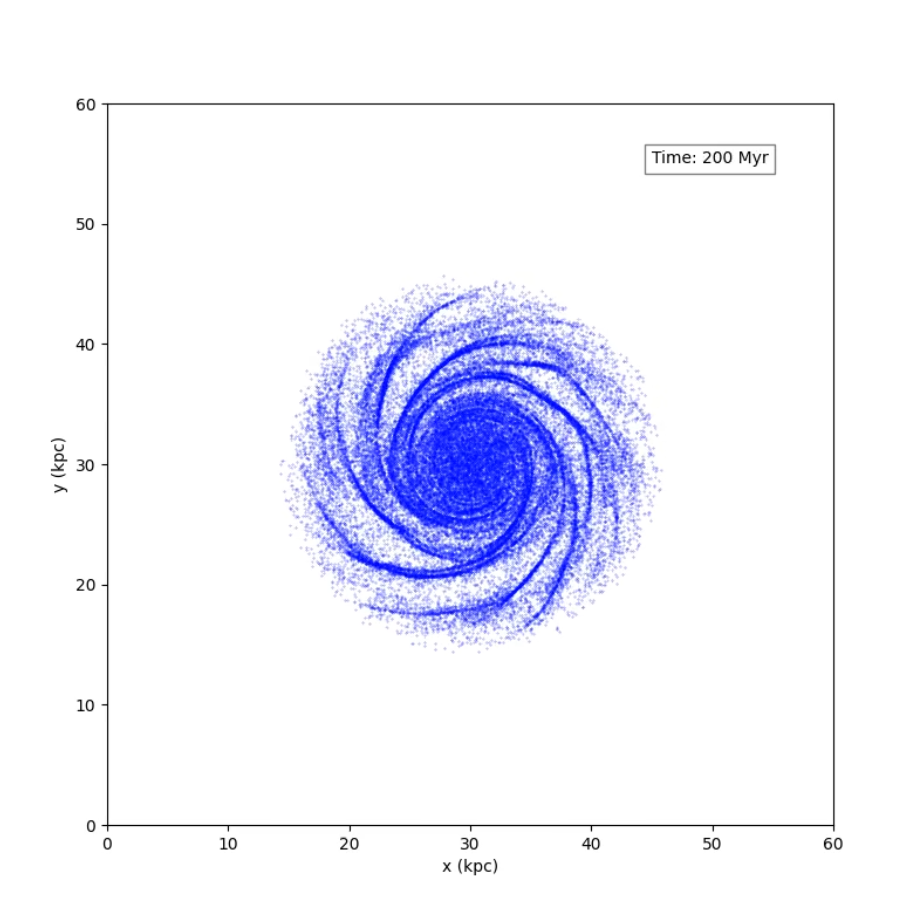
\includegraphics[width=\textwidth]{img/pm/200myr.png}
        \caption{$t=200\,\text{Myr}$}
        \label{fig:spiral-galaxy-evolution-pm-sub4}
    \end{subfigure}

    \caption{Evolution of a spiral galaxy as predicted by the PM method.}
    \label{fig:spiral-galaxy-evolution-pm}
\end{figure}

During the simulation, total energy $E = \textrm{KE} + \textrm{PE}$, angular momentum $\mathbf{l}$, and the $z$-component of the momentum vector $\mathbf{p}$ should stay constant.
The $x$- and $y$-components of momentum change due to the presence of an external gravitational field (representing the halo).
We can verify if this variation satisfies the expected relation
\begin{equation}\label{eq:expected-momentum-change}
    \dot{\mathbf{p}} = \mathbf{F}^\text{ext}
\end{equation}
by finding the initial total momentum $\mathbf{p}(t = 0)$ and incrementing the value of $\mathbf{p}$ in each time-step by $\mathbf{F}^\text{ext}\textrm{DT}$.

The exact calculation of the potential energy \cite{taylor2005classical} using the formula
\begin{equation*}
    \textrm{PE} = -\sum_{i=1}^{N}\sum_{j=i+1}^{N}\frac{G m_i m_j}{r_{ij}}
\end{equation*}
is computationally infeasible considering the $O(N^2)$ cost.
An approximation based on the potential values at mesh points,
\begin{equation*}
    \textrm{PE} \approx \frac{V}{2}\sum_{\mathbf{p}} \rho(\mathbf{x}_\mathbf{p})\phi(\mathbf{x}_\mathbf{p}),
\end{equation*}
is used instead (for derivation refer to \cite{Hockney1988}).
\begin{figure}[htp]
    \centering
    \begin{subfigure}[b]{0.45\textwidth}
        \centering
        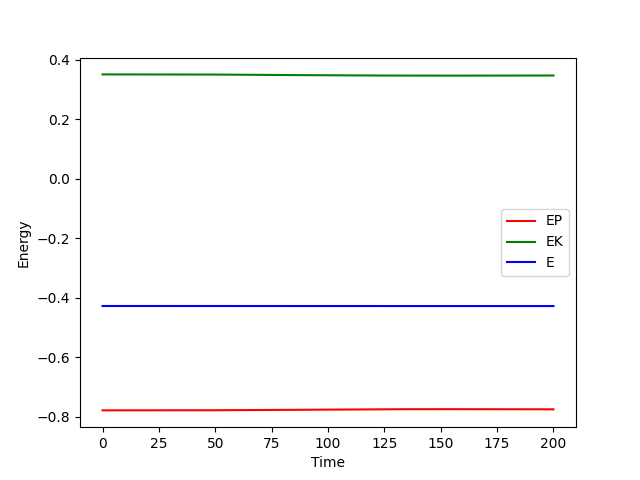
\includegraphics[width=\textwidth]{img/pm/energy.png}
        \caption{Energy}
        \label{fig:physical-quantities-pm-sub1}
    \end{subfigure}
    \hfill
    \begin{subfigure}[b]{0.45\textwidth}
        \centering
        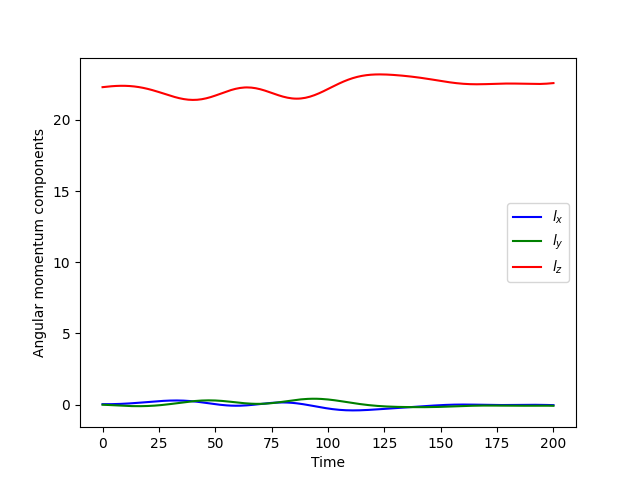
\includegraphics[width=\textwidth]{img/pm/angular-momentum.png}
        \caption{Angular momentum}
        \label{fig:physical-quantities-pm-sub2}
    \end{subfigure}

    \vspace{0.5cm}

    \begin{subfigure}[b]{0.45\textwidth}
        \centering
        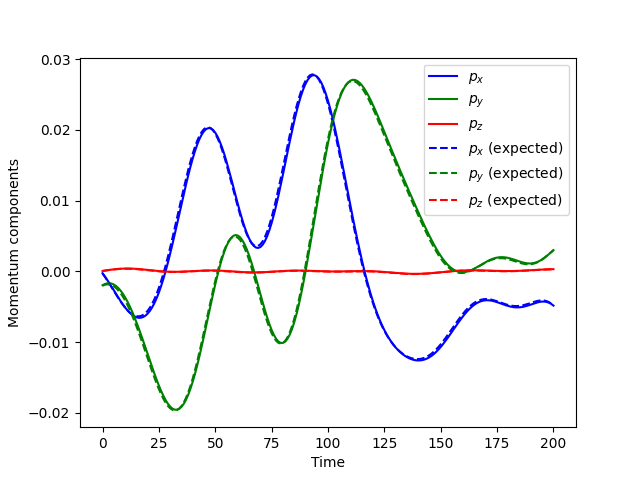
\includegraphics[width=\textwidth]{img/pm/momentum.png}
        \caption{Momentum; broken lines represent the expected momentum following \autoref{eq:expected-momentum-change}}
        \label{fig:physical-quantities-pm-sub3}
    \end{subfigure}

    \caption{Fundamental physical quantities describing the system over time in the PM simulation.
        Time is in Myr and the quantities are expressed in units consistent with \autoref{tab:galaxy-parameters}}
    \label{fig:physical-quantities-pm}
\end{figure}

\subsection{Particle-particle particle-mesh method}
The \PThreeM{} based simulation uses the same parameters as the PM method.
The reference force was calculated using the $S_1$ shape formula (\autoref{eq:s1-reference-force}) with particle diameter $a=3H$.
The cutoff radius was set to $r_e=0.7a$.
One extra free parameter is the \textit{softening length} $\epsilon$ which modifies the universal law of gravitation so that division by zero can be avoided, i.e. the modified law is
\begin{equation*}
    F^\text{soft}_{ij}(r) = \frac{G m_i m_j}{r_{ij}^2 + \epsilon^2}.
\end{equation*}
In the simulation, $\epsilon$ was set arbitrarily to $1.5$ kpc.
The system's evolution is presented in \autoref{fig:spiral-galaxy-evolution-p3m}.
\begin{figure}[htp]
    \centering
    \begin{subfigure}[b]{0.45\textwidth}
        \centering
        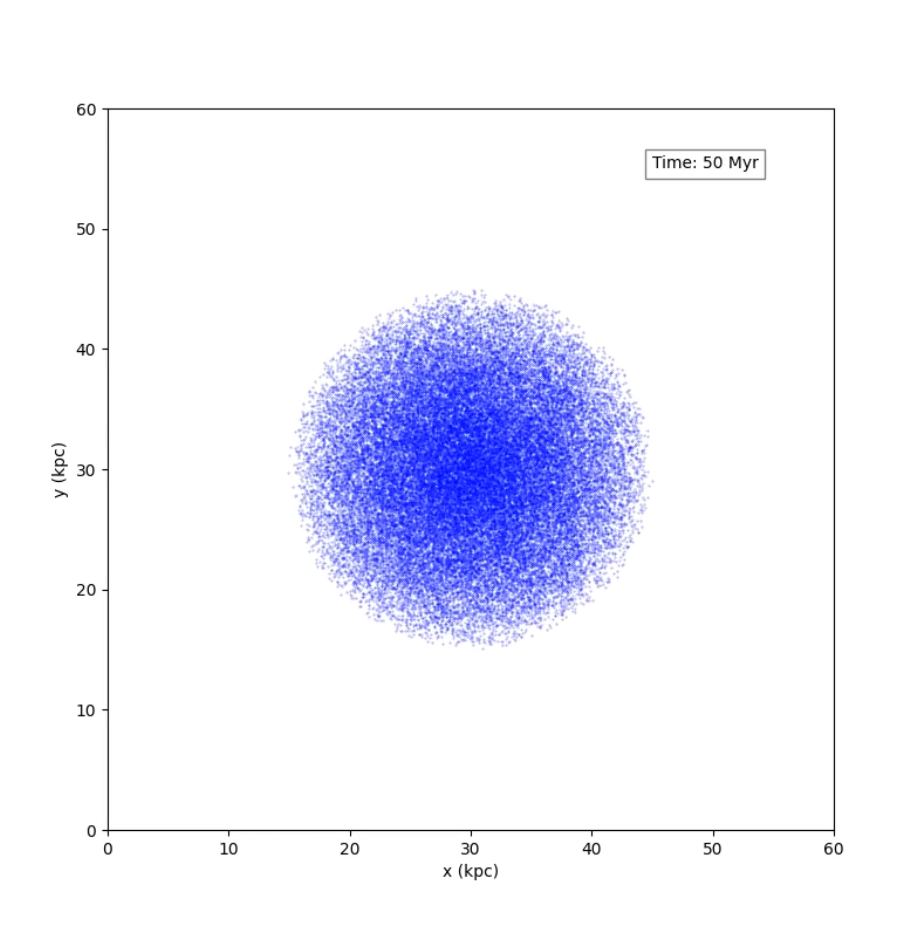
\includegraphics[width=\textwidth]{img/p3m/50myr.png}
        \caption{$t=50\,\text{Myr}$}
        \label{fig:spiral-galaxy-evolution-p3m-sub1}
    \end{subfigure}
    \hfill
    \begin{subfigure}[b]{0.45\textwidth}
        \centering
        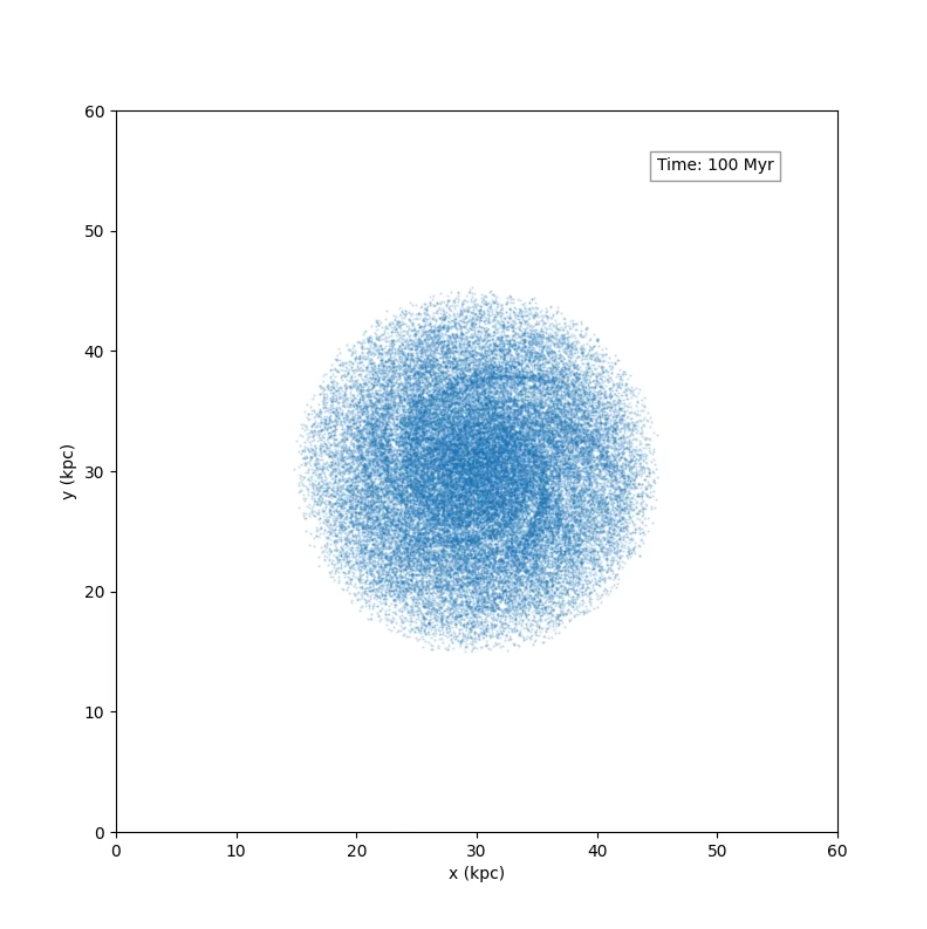
\includegraphics[width=\textwidth]{img/p3m/100myr.png}
        \caption{$t=100\,\text{Myr}$}
        \label{fig:spiral-galaxy-evolution-p3m-sub2}
    \end{subfigure}

    \vspace{0.5cm}

    \begin{subfigure}[b]{0.45\textwidth}
        \centering
        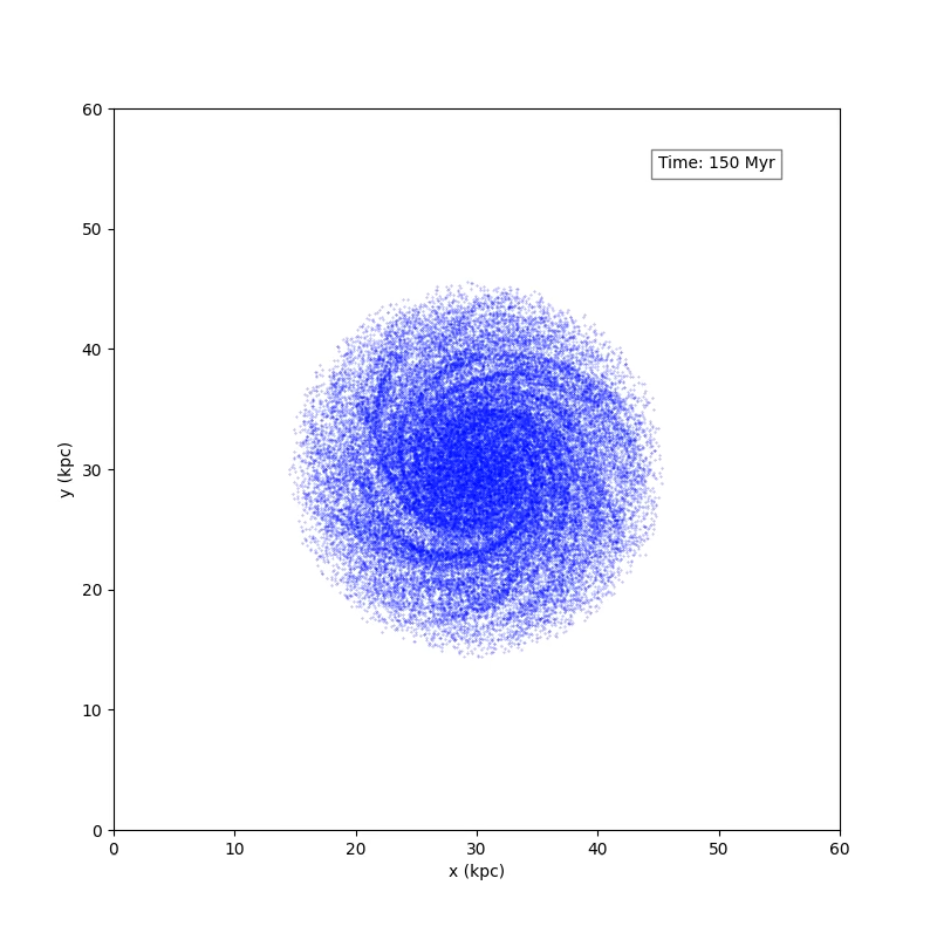
\includegraphics[width=\textwidth]{img/p3m/150myr.png}
        \caption{$t=150\,\text{Myr}$}
        \label{fig:spiral-galaxy-evolution-p3m-sub3}
    \end{subfigure}
    \hfill
    \begin{subfigure}[b]{0.45\textwidth}
        \centering
        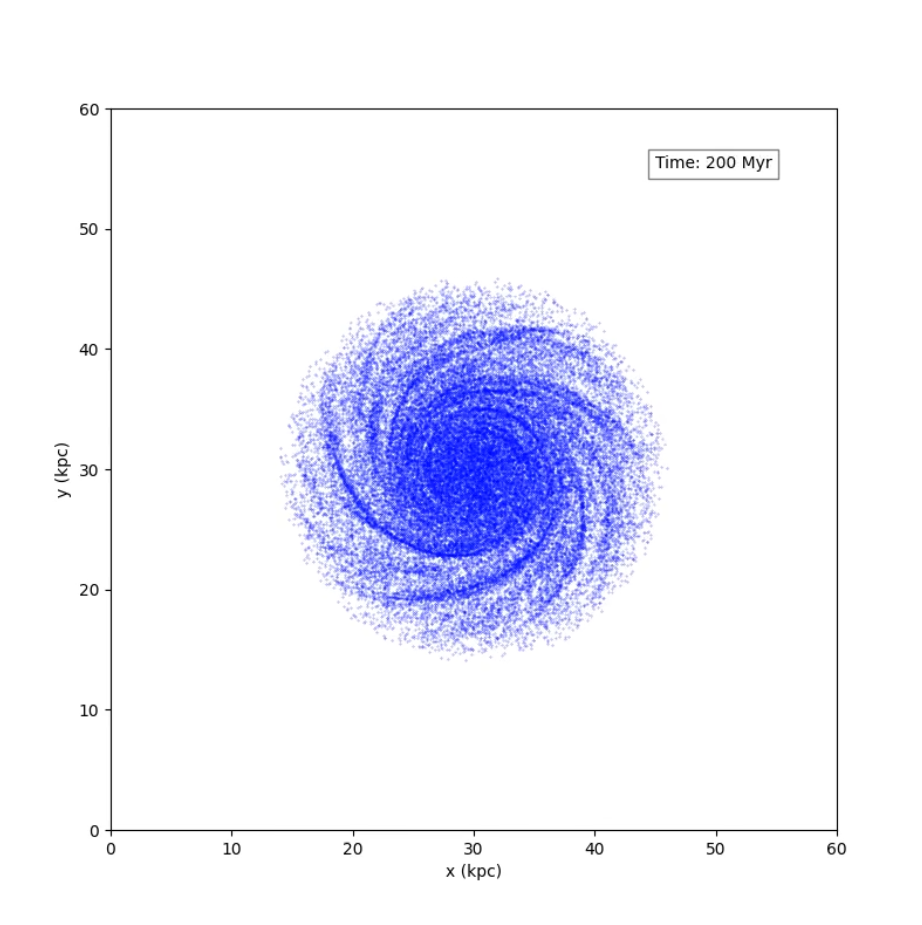
\includegraphics[width=\textwidth]{img/p3m/200myr.png}
        \caption{$t=200\,\text{Myr}$}
        \label{fig:spiral-galaxy-evolution-p3m-sub4}
    \end{subfigure}

    \caption{Evolution of a spiral galaxy as predicted by the \PThreeM{} method.}
    \label{fig:spiral-galaxy-evolution-p3m}
\end{figure}
Graphs of energy, angular momentum, and momentum components vs. time are shown in \autoref{fig:physical-quantities-p3m}.
\begin{figure}[htp]
    \centering
    \begin{subfigure}[b]{0.45\textwidth}
        \centering
        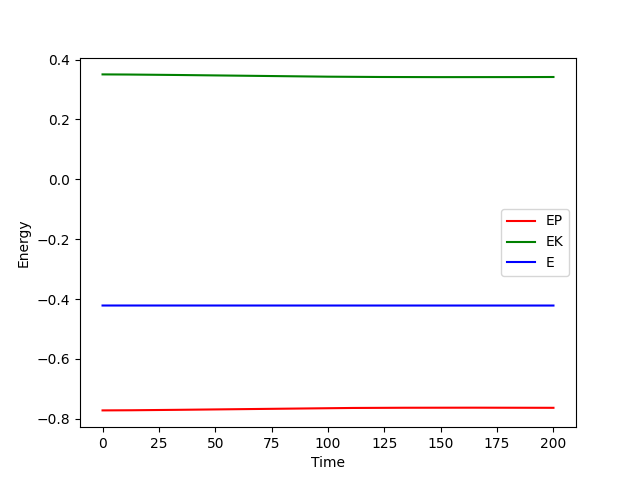
\includegraphics[width=\textwidth]{img/p3m/energy.png}
        \caption{Energy}
        \label{fig:physical-quantities-p3m-sub1}
    \end{subfigure}
    \hfill
    \begin{subfigure}[b]{0.45\textwidth}
        \centering
        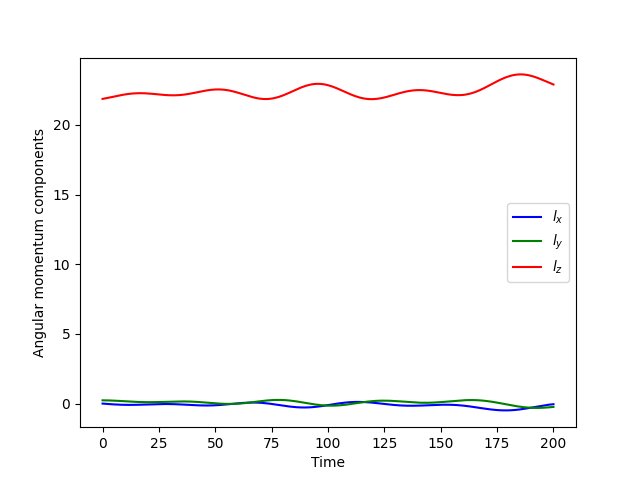
\includegraphics[width=\textwidth]{img/p3m/angular-momentum.png}
        \caption{Angular momentum}
        \label{fig:physical-quantities-p3m-sub2}
    \end{subfigure}

    \vspace{0.5cm}

    \begin{subfigure}[b]{0.45\textwidth}
        \centering
        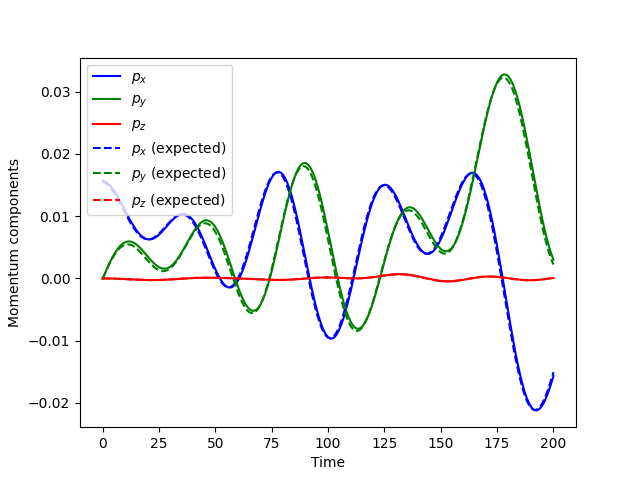
\includegraphics[width=\textwidth]{img/p3m/momentum.png}
        \caption{Momentum; broken lines represent the expected momentum following \autoref{eq:expected-momentum-change}}
        \label{fig:physical-quantities-p3m-sub3}
    \end{subfigure}

    \caption{Fundamental physical quantities describing the system over time in the \PThreeM{} simulation.
        Time is in Myr and the quantities are expressed in units consistent with \autoref{tab:galaxy-parameters}}
    \label{fig:physical-quantities-p3m}
\end{figure}

\subsection{Performance analysis}
The PM and \PThreeM{} methods were implemented exactly as described in the previous sections.
The PM method was developed for both CPU and GPU architectures, using C++ and CUDA C++, respectively, while the \PThreeM{} method is currently available only in the CPU variant.
The implementation relies on external libraries for fast Fourier transform computations: FFTW for the CPU version and cuFFT for the GPU version.
A performance comparison of the PM method was conducted using $N = 2^{16} = 65,536$ particles on a $64 \times 64 \times 64$ mesh with the CIC assignment scheme.
The tests were run on a system equipped with an Intel(R) Core(TM) i7-9750H CPU @ 2.60GHz and an NVIDIA GeForce GTX 1650 GPU. Over 200 iterations, the CPU implementation consistently took around 2.3 seconds, while the GPU implementation reduced this to approximately 1.0 second (excluding data transfer time between host and device).
Notably, the most time-consuming part of the program was unrelated to computation—writing data to disk in text format took nearly 20 seconds.

For the \PThreeM{} method, performance was measured using $N=50,000$ particles on a $128 \times 128 \times 64$ mesh with the TSC assignment scheme.
The total runtime was approximately 1 minute and 30 seconds, with the time distribution among key algorithm components as follows:
\begin{itemize}
    \item HOC table initialization: 12\%
    \item Short-range force calculations: 80\%
    \item PM step: 7.5\%
\end{itemize}
The code is available at \url{https://github.com/AleksyBalazinski/ParticleSimulation} under the MIT license.